\documentclass[10pt,fleqn]{book} % Default font size and left-justified equations
\usepackage[%
    pdftitle={Modélisation systèmes multiphysiques : Modélisation par fonction de transfert et schéma-blocs},
    pdfauthor={Xavier Pessoles}]{hyperref}
%%%%%%%%%%%%%%%%%%%%%%%%%%%%%%%%%%%%%%%%%
% Original author:
% Mathias Legrand (legrand.mathias@gmail.com) with modifications by:
% Vel (vel@latextemplates.com)
% License:
% CC BY-NC-SA 3.0 (http://creativecommons.org/licenses/by-nc-sa/3.0/)
%%%%%%%%%%%%%%%%%%%%%%%%%%%%%%%%%%%%%%%%%

%----------------------------------------------------------------------------------------
%	VARIOUS REQUIRED PACKAGES AND CONFIGURATIONS
%----------------------------------------------------------------------------------------

\usepackage[top=2.5cm,bottom=2cm,left=2cm,right=2cm,headsep=40pt,a4paper]{geometry} % Page margins

\usepackage{graphicx} % Required for including pictures
\graphicspath{{images/}} % Specifies the directory where pictures are stored

\usepackage{lipsum} % Inserts dummy text

\usepackage{tikz} % Required for drawing custom shapes

\usepackage[french]{babel} % English language/hyphenation
\frenchbsetup{StandardLists=true} % Pour éviter la collision babel enumitem pour les listes

\usepackage{enumitem} % Customize lists
\setlist{nolistsep} % Reduce spacing between bullet points and numbered lists

\usepackage{booktabs} % Required for nicer horizontal rules in tables

\usepackage{xcolor} % Required for specifying colors by name
%\definecolor{ocre}{RGB}{243,102,25} % Define the orange color used for highlighting throughout the book
 \definecolor{ocre}{RGB}{49,133,156} % Couleur ''bleue''
\definecolor{violetf}{RGB}{112,48,160} % Couleur ''violet''
\usepackage{enumitem}
\usepackage{pifont} % Pour les dinglist
\usepackage{multicol}
\usepackage{array} % Centrage vertical dans les tableaux

%----------------------------------------------------------------------------------------
%	FONTS
%----------------------------------------------------------------------------------------

\usepackage{avant} % Use the Avantgarde font for headings
%\usepackage{times} % Use the Times font for headings
%\usepackage{mathptmx} % Use the Adobe Times Roman as the default text font together with math symbols from the Sym­bol, Chancery and Com­puter Modern fonts
\usepackage[adobe-utopia]{mathdesign}
\usepackage{microtype} % Slightly tweak font spacing for aesthetics
\usepackage[utf8]{inputenc} % Required for including letters with accents
\usepackage[T1]{fontenc} % Use 8-bit encoding that has 256 glyphs

%----------------------------------------------------------------------------------------
%	BIBLIOGRAPHY AND INDEX
%----------------------------------------------------------------------------------------

\usepackage[style=alphabetic,citestyle=numeric,sorting=nyt,sortcites=true,autopunct=true,babel=hyphen,hyperref=true,abbreviate=false,backref=true,backend=biber]{biblatex}
\addbibresource{bibliography.bib} % BibTeX bibliography file
\defbibheading{bibempty}{}

\usepackage{calc} % For simpler calculation - used for spacing the index letter headings correctly
\usepackage{makeidx} % Required to make an index
\makeindex % Tells LaTeX to create the files required for indexing

%----------------------------------------------------------------------------------------
%	MAIN TABLE OF CONTENTS
%----------------------------------------------------------------------------------------

\usepackage{titletoc} % Required for manipulating the table of contents

\setcounter{tocdepth}{2}     % Dans la table des matieres
\setcounter{secnumdepth}{2}

\contentsmargin{0cm} % Removes the default margin

% Part text styling
\titlecontents{part}[0cm]
{\addvspace{20pt}\centering\large\bfseries}
{}
{}
{}

% Chapter text styling
\titlecontents{chapter}[1.25cm] % Indentation
{\addvspace{12pt}\large\sffamily\bfseries} % Spacing and font options for chapters
{\color{ocre!60}\contentslabel[\Large\thecontentslabel]{1.25cm}\color{ocre}} % Chapter number
{\color{ocre}}  
{\color{ocre!60}\normalsize\;\titlerule*[.5pc]{.}\;\thecontentspage} % Page number

% Section text styling
\titlecontents{section}[1.25cm] % Indentation
{\addvspace{3pt}\sffamily\bfseries} % Spacing and font options for sections
{\color{ocre!60}\contentslabel[\thecontentslabel]{1.25cm} \color{ocre}} % Section number
{\color{ocre}}
{\hfill\color{ocre!60}\thecontentspage} % Page number
[]

% Subsection text styling
\titlecontents{subsection}[1.25cm] % Indentation
{\addvspace{1pt}\sffamily\small} % Spacing and font options for subsections
{\contentslabel[\thecontentslabel]{1.25cm}} % Subsection number
{}
{\ \titlerule*[.5pc]{.}\;\thecontentspage} % Page number
[]


% Subsection text styling
\titlecontents{subsubsection}[1.25cm] % Indentation
{\addvspace{1pt}\sffamily\small} % Spacing and font options for subsections
{\contentslabel[\thecontentslabel]{1.25cm}} % Subsection number
{}
{\ \titlerule*[.5pc]{.}\;\thecontentspage} % Page number
[]

% List of figures
\titlecontents{figure}[0em]
{\addvspace{-5pt}\sffamily}
{\thecontentslabel\hspace*{1em}}
{}
{\ \titlerule*[.5pc]{.}\;\thecontentspage}
[]

% List of tables
\titlecontents{table}[0em]
{\addvspace{-5pt}\sffamily}
{\thecontentslabel\hspace*{1em}}
{}
{\ \titlerule*[.5pc]{.}\;\thecontentspage}
[]

%----------------------------------------------------------------------------------------
%	MINI TABLE OF CONTENTS IN PART HEADS
%----------------------------------------------------------------------------------------

% Chapter text styling
\titlecontents{lchapter}[0em] % Indenting
{\addvspace{15pt}\large\sffamily\bfseries} % Spacing and font options for chapters
{\color{ocre}\contentslabel[\Large\thecontentslabel]{1.25cm}\color{ocre}} % Chapter number
{}  
{\color{ocre}\normalsize\sffamily\bfseries\;\titlerule*[.5pc]{.}\;\thecontentspage} % Page number

% Section text styling
\titlecontents{lsection}[0em] % Indenting
{\sffamily\small} % Spacing and font options for sections
{\contentslabel[\thecontentslabel]{1.25cm}} % Section number
{}
{}

% Subsection text styling
\titlecontents{lsubsection}[.5em] % Indentation
{\normalfont\footnotesize\sffamily} % Font settings
{}
{}
{}

%----------------------------------------------------------------------------------------
%	PAGE HEADERS
%----------------------------------------------------------------------------------------

\usepackage{fancyhdr} % Required for header and footer configuration



\pagestyle{fancy}
 \renewcommand{\headrulewidth}{0pt}
 \fancyhead{}
 \fancyhead[L]{%
 \noindent\begin{minipage}[c]{2.6cm}%
 
\includegraphics[width=2cm]{png/logo_lycee.png}%
 \end{minipage}}

\fancyhead[C]{\rule{8cm}{.5pt}}

 \fancyhead[R]{%
 \noindent\begin{minipage}[c]{3cm}
 \begin{flushright}
 \footnotesize{\textit{\textsf{\xxtete}}}%
 \end{flushright}
 \end{minipage}
}


\fancyfoot[C]{\rule{12cm}{.5pt}}
\renewcommand{\footrulewidth}{0.2pt}
\fancyfoot[C]{\footnotesize{\bfseries \thepage}}
\fancyfoot[L]{ 
\begin{minipage}[c]{.4\linewidth}
\noindent\footnotesize{{\xxauteur}}
\end{minipage}}


\fancyfoot[R]{\footnotesize{\xxpied}
\ifthenelse{\isodd{\value{page}}}{
\begin{tikzpicture}[overlay]
\node[shape=rectangle, 
      rounded corners = .25 cm,
	  draw= ocre,
	  line width=2pt, 
	  fill = ocre!10,
	  minimum width  = 2.5cm,
	  minimum height = 3cm,] at (\xxposongletx,\xxposonglety) {};
\node at (\xxposonglettext,\xxposonglety) {\rotatebox{90}{\textbf{\large\color{ocre}{\xxonglet}}}};
%{};
\end{tikzpicture}}{}
}
%
%
%
% Removes the header from odd empty pages at the end of chapters
\makeatletter
\renewcommand{\cleardoublepage}{
\clearpage\ifodd\c@page\else
\hbox{}
\vspace*{\fill}
\thispagestyle{empty}
\newpage
\fi}

\fancypagestyle{plain}{%
\fancyhf{} % vide l’en-tête et le pied~de~page.
%\fancyfoot[C]{\bfseries \thepage} % numéro de la page en cours en gras
% et centré en pied~de~page.
\fancyfoot[R]{\footnotesize{\xxpied}}
\fancyfoot[C]{\rule{12cm}{.5pt}}
\renewcommand{\footrulewidth}{0.2pt}
\fancyfoot[C]{\footnotesize{\bfseries \thepage}}
\fancyfoot[L]{ 
\begin{minipage}[c]{.4\linewidth}
\noindent\footnotesize{{\xxauteur}}
\end{minipage}}}



%----------------------------------------------------------------------------------------
%	THEOREM STYLES
%----------------------------------------------------------------------------------------

% Conflit avec la police adobe
%\usepackage{amsmath,amsfonts,amssymb,amsthm} % For math equations, theorems, symbols, etc
\usepackage{amsmath,amsthm}

\newcommand{\intoo}[2]{\mathopen{]}#1\,;#2\mathclose{[}}
\newcommand{\ud}{\mathop{\mathrm{{}d}}\mathopen{}}
\newcommand{\intff}[2]{\mathopen{[}#1\,;#2\mathclose{]}}
%\newtheorem{notation}{Notation}[chapter]
\newtheorem{notation}{Notation}[section]

% Boxed/framed environments
\newtheoremstyle{ocrenumbox}% % Theorem style name
{0pt}% Space above
{0pt}% Space below
{\normalfont}% % Body font
{}% Indent amount
{\small\bf\sffamily\color{ocre}}% % Theorem head font
{\;}% Punctuation after theorem head
{0.25em}% Space after theorem head
{\small\sffamily\color{ocre}\thmname{#1}\nobreakspace\thmnumber%{\@ifnotempty{#1}{}\@upn{#2}}% Theorem text (e.g. Theorem 2.1)
\thmnote{\nobreakspace\the\thm@notefont\sffamily\bfseries\color{black}---\nobreakspace#3.}} % Optional theorem note
\renewcommand{\qedsymbol}{$\blacksquare$}% Optional qed square


% Boite pour les corriges
\newtheoremstyle{correctionbox}% % Theorem style name
{0pt}% Space above
{0pt}% Space below
{\normalfont}% % Body font
{}% Indent amount
{\small\bf\sffamily\color{violet}}% % Theorem head font
{\;}% Punctuation after theorem head
{0.25em}% Space after theorem head
{\small\sffamily\color{ocre}\thmname{#1}\nobreakspace\thmnumber%{\@ifnotempty{#1}{}\@upn{#2}}% Theorem text (e.g. Theorem 2.1)
\thmnote{\nobreakspace\the\thm@notefont\sffamily\bfseries\color{black}---\nobreakspace#3.}} % Optional theorem note
\renewcommand{\qedsymbol}{$\blacksquare$}% Optional qed square



\newtheoremstyle{blacknumex}% Theorem style name
{5pt}% Space above
{5pt}% Space below
{\normalfont}% Body font
{} % Indent amount
{\small\bf\sffamily}% Theorem head font
{\;}% Punctuation after theorem head
{0.25em}% Space after theorem head
{\small\sffamily{\tiny\ensuremath{\blacksquare}}\nobreakspace\thmname{#1}\nobreakspace\thmnumber%{\@ifnotempty{#1}{}\@upn{#2}}% Theorem text (e.g. Theorem 2.1)
\thmnote{\nobreakspace\the\thm@notefont\sffamily\bfseries---\nobreakspace#3.}}% Optional theorem note

\newtheoremstyle{blacknumbox} % Theorem style name
{0pt}% Space above
{0pt}% Space below
{\normalfont}% Body font
{}% Indent amount
{\small\bf\sffamily}% Theorem head font
{\;}% Punctuation after theorem head
{0.25em}% Space after theorem head
{\small\sffamily\thmname{#1}\nobreakspace 
\thmnote{\nobreakspace\the\thm@notefont\sffamily\bfseries---\nobreakspace#3.}}% Optional theorem note

% Non-boxed/non-framed environments
\newtheoremstyle{ocrenum}% % Theorem style name
{5pt}% Space above
{5pt}% Space below
{\normalfont}% % Body font
{}% Indent amount
{\small\bf\sffamily\color{ocre}}% % Theorem head font
{\;}% Punctuation after theorem head
{0.25em}% Space after theorem head
{\small\sffamily\color{ocre}\thmname{#1}\nobreakspace%\thmnumber{\@ifnotempty{#1}{}\@upn{#2}}% Theorem text (e.g. Theorem 2.1)
\thmnote{\nobreakspace\the\thm@notefont\sffamily\bfseries\color{black}---\nobreakspace#3.}} % Optional theorem note
\renewcommand{\qedsymbol}{$\blacksquare$}% Optional qed square
\makeatother

% Environnement pour les titres de parties
\newtheoremstyle{partiebox} 
{0pt}% Space above
{0pt}% Space below
{\normalfont}% Body font
{}% Indent amount
{\small\bf\sffamily}% Theorem head font
{\;}% Punctuation after theorem head
{0.25em}% Space after theorem head




% Defines the theorem text style for each type of theorem to one of the three styles above
\newcounter{dummy} 
\numberwithin{dummy}{section}
\theoremstyle{ocrenumbox}
%\newtheorem{theoremeT}[dummy]{Théorème}
\newtheorem{theoremeT}[dummy]{Théorème}
\newtheorem{resultatT}[dummy]{Résultat}
\newtheorem{savoirT}[dummy]{Savoir}
\newtheorem{methodeT}[dummy]{Méthode}
\newtheorem{objectifT}[dummy]{Objectif}
%\newtheorem{problem}{Problem}[chapter]
\newtheorem{problem}{Problem}[section]
%\newtheorem{exerciseT}{Exercise}[chapter]
\newtheorem{exerciseT}{Exercice}[section]

\theoremstyle{blacknumex}
%\newtheorem{exampleT}{Example}[chapter]
\newtheorem{exempleT}{Exemple}[section]
\newtheorem{termT}{Terminal\\}[section]
\newtheorem{pyT}{Python\\}[section]
\newtheorem{sciT}{Scilab\\}[section]
\newtheorem{pseudoT}{Pseudo Code\\}[section]
\newtheorem{sqlT}{SQL\\}[section]

\theoremstyle{blacknumbox}
%\newtheorem{vocabulary}{Vocabulary}[chapter]
\newtheorem{vocabulary}{Vocabulaire}[section]
%\newtheorem{definitionT}{Definition}[section]
\newtheorem{definitionT}{Définition}[section]
\newtheorem{rappelT}{Rappel}[section]
\newtheorem{demoT}{Démonstration}[section]
\newtheorem{corollaryT}[dummy]{Corollaire}
\newtheorem{hypoT}{Hypothèse(s)}

\theoremstyle{ocrenum}
\newtheorem{proposition}[dummy]{Proposition}

\theoremstyle{partiebox}
\newtheorem{titrepartieT}[]{}
\newtheorem{titrechapitreT}[]{}

\theoremstyle{correctionbox}
\newtheorem{correctionT}[dummy]{\color{violet}{Correction}}

%----------------------------------------------------------------------------------------
%	DEFINITION OF COLORED BOXES
%----------------------------------------------------------------------------------------

\RequirePackage[framemethod=tikz]{mdframed} % Required for creating the theorem, definition, exercise and corollary boxes

% Theorem box
\newmdenv[skipabove=7pt,
skipbelow=7pt,
backgroundcolor=ocre!10,
linecolor=ocre,
innerleftmargin=5pt,
innerrightmargin=5pt,
innertopmargin=5pt,
leftmargin=0cm,
rightmargin=0cm,
innerbottommargin=5pt]{tBox}


% Correction
\newmdenv[skipabove=7pt,
skipbelow=7pt,
backgroundcolor=violet!10,
linecolor=violet,
innerleftmargin=5pt,
innerrightmargin=5pt,
innertopmargin=5pt,
leftmargin=0cm,
rightmargin=0cm,
innerbottommargin=5pt]{coBox}


% Exercise box	  
\newmdenv[skipabove=7pt,
skipbelow=7pt,
rightline=false,
leftline=true,
topline=false,
bottomline=false,
backgroundcolor=ocre!10,
linecolor=ocre,
innerleftmargin=5pt,
innerrightmargin=5pt,
innertopmargin=5pt,
innerbottommargin=5pt,
leftmargin=0cm,
rightmargin=0cm,
linewidth=4pt]{eBox}	

% Definition box
\newmdenv[skipabove=7pt,
skipbelow=7pt,
rightline=false,
leftline=true,
topline=false,
bottomline=false,
backgroundcolor=ocre!10,
linecolor=ocre,
innerleftmargin=5pt,
innerrightmargin=5pt,
innertopmargin=0pt,
leftmargin=0cm,
rightmargin=0cm,
linewidth=4pt,
innerbottommargin=0pt]{dBox}	

% Demonstration box
\newmdenv[skipabove=7pt,
skipbelow=7pt,
rightline=false,
leftline=true,
topline=false,
bottomline=false,
%backgroundcolor=ocre!10,
linecolor=ocre,
innerleftmargin=5pt,
innerrightmargin=5pt,
innertopmargin=0pt,
leftmargin=0cm,
rightmargin=0cm,
linewidth=4pt,
innerbottommargin=0pt]{demoBox}	

% Corollary box
\newmdenv[skipabove=7pt,
skipbelow=7pt,
rightline=false,
leftline=true,
topline=false,
bottomline=false,
linecolor=gray,
backgroundcolor=black!5,
innerleftmargin=5pt,
innerrightmargin=5pt,
innertopmargin=5pt,
leftmargin=0cm,
rightmargin=0cm,
linewidth=4pt,
innerbottommargin=5pt]{cBox}


% Hypothèses
\newmdenv[skipabove=7pt,
skipbelow=7pt,
rightline=false,
leftline=true,
topline=false,
bottomline=false,
linecolor=gray,
backgroundcolor=black!5,
innerleftmargin=5pt,
innerrightmargin=5pt,
innertopmargin=5pt,
leftmargin=0cm,
rightmargin=0cm,
linewidth=4pt,
innerbottommargin=5pt]{hyBox}


% Boite pour le titre de la partie (pBox)
\newmdenv[skipabove=7pt,
skipbelow=7pt,
rightline=true,
leftline=false,
topline=false,
bottomline=false,
linecolor=ocre,
backgroundcolor=none,
innerleftmargin=5pt,
innerrightmargin=5pt,
innertopmargin=5pt,
leftmargin=0cm,
rightmargin=0cm,
linewidth=4pt,
innerbottommargin=5pt]{pBox}

% Boite pour le titre du chapitre (chBox)
\newmdenv[skipabove=7pt,
skipbelow=7pt,
rightline=false,
leftline=true,
topline=false,
bottomline=false,
linecolor=ocre,
%backgroundcolor=black!5,
innerleftmargin=5pt,
innerrightmargin=5pt,
innertopmargin=5pt,
leftmargin=0cm,
rightmargin=0cm,
linewidth=4pt,
innerbottommargin=5pt]{chBox}


% Boite pour les exemples
\newmdenv[skipabove=7pt,
skipbelow=7pt,
rightline=false,
leftline=true,
topline=false,
bottomline=false,
linecolor=gray,
backgroundcolor=white,
innerleftmargin=5pt,
innerrightmargin=5pt,
innertopmargin=5pt,
leftmargin=0cm,
rightmargin=0cm,
linewidth=4pt,
innerbottommargin=5pt]{exBox}

% Boite pour le terminal
\newmdenv[skipabove=7pt,
skipbelow=7pt,
rightline=false,
leftline=true,
topline=false,
bottomline=false,
linecolor=gray,
backgroundcolor=white,
innerleftmargin=5pt,
innerrightmargin=5pt,
innertopmargin=5pt,
leftmargin=0cm,
rightmargin=0cm,
linewidth=4pt,
innerbottommargin=5pt]{termBox}


% Boite pour Python
\newmdenv[skipabove=7pt,
skipbelow=7pt,
rightline=false,
leftline=true,
topline=false,
bottomline=false,
linecolor=gray,
backgroundcolor=white,
innerleftmargin=5pt,
innerrightmargin=5pt,
innertopmargin=0pt,
leftmargin=0cm,
rightmargin=0cm,
linewidth=4pt,
innerbottommargin=5pt]{pyBox}

% Boite pour scilab
\newmdenv[skipabove=7pt,
skipbelow=7pt,
rightline=false,
leftline=true,
topline=false,
bottomline=false,
linecolor=gray,
backgroundcolor=white,
innerleftmargin=5pt,
innerrightmargin=5pt,
innertopmargin=5pt,
leftmargin=0cm,
rightmargin=0cm,
linewidth=4pt,
innerbottommargin=5pt]{sciBox}


% Boite pour pseudo
\newmdenv[skipabove=7pt,
skipbelow=7pt,
rightline=false,
leftline=true,
topline=false,
bottomline=false,
linecolor=gray,
backgroundcolor=white,
innerleftmargin=5pt,
innerrightmargin=5pt,
innertopmargin=5pt,
leftmargin=0cm,
rightmargin=0cm,
linewidth=4pt,
innerbottommargin=5pt]{pseudoBox}

% Boite pour pseudo
\newmdenv[skipabove=7pt,
skipbelow=7pt,
rightline=false,
leftline=true,
topline=false,
bottomline=false,
linecolor=gray,
backgroundcolor=white,
innerleftmargin=5pt,
innerrightmargin=5pt,
innertopmargin=5pt,
leftmargin=0cm,
rightmargin=0cm,
linewidth=4pt,
innerbottommargin=5pt]{sqlBox}


% Creates an environment for each type of theorem and assigns it a theorem text style from the "Theorem Styles" section above and a colored box from above
\newenvironment{theorem}{\begin{tBox}\begin{theoremeT}}{\end{theoremeT}\end{tBox}}
\newenvironment{resultat}{\begin{tBox}\begin{resultatT}}{\end{resultatT}\end{tBox}}
\newenvironment{methode}{\begin{tBox}\begin{methodeT}}{\end{methodeT}\end{tBox}}
\newenvironment{savoir}{\begin{tBox}\begin{savoirT}}{\end{savoirT}\end{tBox}}
\newenvironment{obj}{\begin{tBox}\begin{objectifT}}{\end{objectifT}\end{tBox}}
\newenvironment{corrige}{\begin{coBox}\begin{correctionT}}{\end{correctionT}\end{coBox}}
\newenvironment{exercise}{\begin{eBox}\begin{exerciseT}}{\hfill{\color{ocre}\tiny\ensuremath{\blacksquare}}\end{exerciseT}\end{eBox}}				  
\newenvironment{exercice}{\begin{eBox}\begin{exerciseT}}{\hfill{\color{ocre}\tiny\ensuremath{\blacksquare}}\end{exerciseT}\end{eBox}}				  

\newenvironment{definition}{\begin{dBox}\begin{definitionT}}{\end{definitionT}\end{dBox}}	
\newenvironment{rappel}{\begin{dBox}\begin{rappelT}}{\end{rappelT}\end{dBox}}	
\newenvironment{defi}{\begin{dBox}\begin{definitionT}}{\end{definitionT}\end{dBox}}	
\newenvironment{demo}{\begin{demoBox}\begin{demoT}}{\end{demoT}\end{demoBox}}	
%\newenvironment{exemple}{\begin{exempleT}}{\hfill{\tiny\ensuremath{\blacksquare}}\end{exempleT}}		
\newenvironment{corollary}{\begin{cBox}\begin{corollaryT}}{\end{corollaryT}\end{cBox}}
\newenvironment{hypo}{\begin{hyBox}\begin{hypoT}}{\end{hypoT}\end{hyBox}}	\newenvironment{exemple}{\begin{exBox}\begin{exempleT}}{\hfill{\tiny\ensuremath{\blacksquare}}\end{exempleT}\end{exBox}}	
\newenvironment{titrepartie}{\begin{pBox}\begin{titrepartieT}}{\end{titrepartieT}\end{pBox}}	
\newenvironment{titrechapitre}{\begin{chBox}\begin{titrechapitreT}}{\end{titrechapitreT}\end{chBox}}	

\newenvironment{term}{ \begin{termBox}\begin{termT}}{\end{termT}\end{termBox}}
\newenvironment{py}{ \begin{pyBox}\begin{pyT}}{\end{pyT}\end{pyBox}}
\newenvironment{sci}{ \begin{sciBox}\begin{sciT}}{\end{sciT}\end{sciBox}}
\newenvironment{pseudo}{ \begin{pseudoBox}\begin{pseudoT}}{\end{pseudoT}\end{pseudoBox}}
\newenvironment{envsql}{ \begin{sqlBox}\begin{sqlT}}{\end{sqlT}\end{sqlBox}}


%----------------------------------------------------------------------------------------
%	REMARK ENVIRONMENT
%----------------------------------------------------------------------------------------

\newenvironment{remark}{\par\vspace{10pt}\small % Vertical white space above the remark and smaller font size
\begin{list}{}{
\leftmargin=35pt % Indentation on the left
\rightmargin=25pt}\item\ignorespaces % Indentation on the right
\makebox[-2.5pt]{\begin{tikzpicture}[overlay]
\node[draw=ocre!60,line width=1pt,circle,fill=ocre!25,font=\sffamily\bfseries,inner sep=2pt,outer sep=0pt] at (-15pt,0pt){\textcolor{ocre}{R}};\end{tikzpicture}} % Orange R in a circle
\advance\baselineskip -1pt}{\end{list}\vskip5pt} % Tighter line spacing and white space after remark

\newenvironment{rem}{\par\vspace{10pt}\small % Vertical white space above the remark and smaller font size
\begin{list}{}{
\leftmargin=35pt % Indentation on the left
\rightmargin=25pt}\item\ignorespaces % Indentation on the right
\makebox[-2.5pt]{\begin{tikzpicture}[overlay]
\node[draw=ocre!60,line width=1pt,circle,fill=ocre!25,font=\sffamily\bfseries,inner sep=2pt,outer sep=0pt] at (-15pt,0pt){\textcolor{ocre}{R}};\end{tikzpicture}} % Orange R in a circle
\advance\baselineskip -1pt}{\end{list}\vskip5pt} % Tighter line spacing and white space after remark


\newenvironment{warn}{\par\vspace{10pt}\small % Vertical white space above the remark and smaller font size
\begin{list}{}{
\leftmargin=35pt % Indentation on the left
\rightmargin=25pt}\item\ignorespaces % Indentation on the right
\makebox[-2.5pt]{\begin{tikzpicture}[overlay]
\node[draw=red!60,line width=1pt,circle,fill=red!25,font=\sffamily\bfseries,inner sep=2pt,outer sep=0pt] at (-15pt,0pt){\textcolor{black}{!}};\end{tikzpicture}} % Point d'exclamation dans un cercle
\advance\baselineskip -1pt}{\end{list}\vskip5pt} % Tighter line spacing and white space after remark


%----------------------------------------------------------------------------------------
%	SECTION NUMBERING IN THE MARGIN
%----------------------------------------------------------------------------------------
\setcounter{secnumdepth}{3}
\setcounter{tocdepth}{2}



\makeatletter
\renewcommand{\@seccntformat}[1]{\llap{\textcolor{ocre}{\csname the#1\endcsname}\hspace{1em}}}                    
\renewcommand{\section}{\@startsection{section}{1}{\z@}
{-4ex \@plus -1ex \@minus -.4ex}
{1ex \@plus.2ex }
{\normalfont\large\sffamily\bfseries}}
\renewcommand{\subsection}{\@startsection {subsection}{2}{\z@}
{-3ex \@plus -0.1ex \@minus -.4ex}
{0.5ex \@plus.2ex }
{\normalfont\sffamily\bfseries}}
\renewcommand{\subsubsection}{\@startsection {subsubsection}{3}{\z@}
{-2ex \@plus -0.1ex \@minus -.2ex}
{.2ex \@plus.2ex }
{\normalfont\small\sffamily\bfseries}}                        
\renewcommand\paragraph{\@startsection{paragraph}{4}{\z@}
{-2ex \@plus-.2ex \@minus .2ex}
{.1ex}
{\normalfont\small\sffamily\bfseries}}

%----------------------------------------------------------------------------------------
%	PART HEADINGS
%----------------------------------------------------------------------------------------


%----------------------------------------------------------------------------------------
%	CHAPTER HEADINGS
%----------------------------------------------------------------------------------------

% \newcommand{\thechapterimage}{}%
% \newcommand{\chapterimage}[1]{\renewcommand{\thechapterimage}{#1}}%
% \def\@makechapterhead#1{%
% {\parindent \z@ \raggedright \normalfont
% \ifnum \c@secnumdepth >\m@ne
% \if@mainmatter
% \begin{tikzpicture}[remember picture,overlay]
% \node at (current page.north west)
% {\begin{tikzpicture}[remember picture,overlay]
% \node[anchor=north west,inner sep=0pt] at (0,0) {\includegraphics[width=\paperwidth]{\thechapterimage}};
% \draw[anchor=west] (\Gm@lmargin,-9cm) node [line width=2pt,rounded corners=15pt,draw=ocre,fill=white,fill opacity=0.5,inner sep=15pt]{\strut\makebox[22cm]{}};
% \draw[anchor=west] (\Gm@lmargin+.3cm,-9cm) node {\huge\sffamily\bfseries\color{black}\thechapter. #1\strut};
% \end{tikzpicture}};
% \end{tikzpicture}
% \else
% \begin{tikzpicture}[remember picture,overlay]
% \node at (current page.north west)
% {\begin{tikzpicture}[remember picture,overlay]
% \node[anchor=north west,inner sep=0pt] at (0,0) {\includegraphics[width=\paperwidth]{\thechapterimage}};
% \draw[anchor=west] (\Gm@lmargin,-9cm) node [line width=2pt,rounded corners=15pt,draw=ocre,fill=white,fill opacity=0.5,inner sep=15pt]{\strut\makebox[22cm]{}};
% \draw[anchor=west] (\Gm@lmargin+.3cm,-9cm) node {\huge\sffamily\bfseries\color{black}#1\strut};
% \end{tikzpicture}};
% \end{tikzpicture}
% \fi\fi\par\vspace*{270\p@}}}

%-------------------------------------------

\def\@makeschapterhead#1{%
\begin{tikzpicture}[remember picture,overlay]
\node at (current page.north west)
{\begin{tikzpicture}[remember picture,overlay]
\node[anchor=north west,inner sep=0pt] at (0,0) {\includegraphics[width=\paperwidth]{\thechapterimage}};
\draw[anchor=west] (\Gm@lmargin,-9cm) node [line width=2pt,rounded corners=15pt,draw=ocre,fill=white,fill opacity=0.5,inner sep=15pt]{\strut\makebox[22cm]{}};
\draw[anchor=west] (\Gm@lmargin+.3cm,-9cm) node {\huge\sffamily\bfseries\color{black}#1\strut};
\end{tikzpicture}};
\end{tikzpicture}
\par\vspace*{270\p@}}
\makeatother

%----------------------------------------------------------------------------------------
%	HYPERLINKS IN THE DOCUMENTS
%----------------------------------------------------------------------------------------


\hypersetup{hidelinks,backref=true,pagebackref=true,hyperindex=true,colorlinks=false,breaklinks=true,urlcolor= ocre,bookmarks=true,bookmarksopen=false,pdftitle={Title},pdfauthor={Author}}
\usepackage{bookmark}
\bookmarksetup{
open,
numbered,
addtohook={%
\ifnum\bookmarkget{level}=0 % chapter
\bookmarksetup{bold}%
\fi
\ifnum\bookmarkget{level}=-1 % part
\bookmarksetup{color=ocre,bold}%
\fi
}
}

%----------------------------------------------------------------------------------------
%	
%----------------------------------------------------------------------------------------

\newcommand{\thechapterimage}{}%
\newcommand{\chapterimage}[1]{\renewcommand{\thechapterimage}{#1}}%
\def\@makechapterhead#1{%
{\parindent \z@ \raggedright \normalfont
\begin{tikzpicture}[remember picture,overlay]
\node at (current page.north west)
{\begin{tikzpicture}[remember picture,overlay]
\node[anchor=north west,inner sep=0pt] at (0,0) {\includegraphics[width=\paperwidth]{\thechapterimage}};
%\draw[anchor=west] (\Gm@lmargin,-9cm) node [line width=2pt,rounded corners=15pt,draw=ocre,fill=white,fill opacity=0.5,inner sep=15pt]{\strut\makebox[22cm]{}};
%\draw[anchor=west] (\Gm@lmargin+.3cm,-9cm) node {\huge\sffamily\bfseries\color{black}\thechapter. #1\strut};
\end{tikzpicture}};
\end{tikzpicture}
\par\vspace*{270\p@}
}}

 \newcounter{exo}


\makeatletter             
\renewcommand{\subparagraph}{\@startsection{exo}{5}{\z@}%
                                    {-2ex \@plus-.2ex \@minus .2ex}%
                                    {0ex}%               
{\normalfont\bfseries Question \hspace{.7cm} }}
\makeatother
\renewcommand{\thesubparagraph}{\arabic{subparagraph}} 
\makeatletter


%%%% Environnement pour inclure du code
\usepackage{textcomp}
\usepackage[french]{algorithm2e}
\usepackage{listings}
\lstloadlanguages{R}   % pour regler les pb d accent utf8 dans les codes
\lstset{language=R} % pour regler les pb d accent utf8 dans les codes
\renewcommand{\lstlistlistingname}{Listings}
\renewcommand{\lstlistingname}{Listing}

\SetKwBlock{Fonction}{Début Fonction}{Fin Fonction}
\SetKwComment{Comment}{start}{end}

\definecolor{Bleu}{rgb}{0.1,0.1,1.0}
\definecolor{Noir}{rgb}{0,0,0}
\definecolor{Grau}{rgb}{0.5,0.5,0.5}
\definecolor{DunkelGrau}{rgb}{0.15,0.15,0.15}
\definecolor{Hellbraun}{rgb}{0.5,0.25,0.0}
\definecolor{Magenta}{rgb}{1.0,0.0,1.0}
\definecolor{Gris}{gray}{0.5}
\definecolor{Vert}{rgb}{0,0.5,0}
\definecolor{SourceHintergrund}{rgb}{1,1.0,0.95}


\lstnewenvironment{python}[1][]{
\lstset{
%escapeinside={\%*}{*)},
inputencoding=utf8,   % pour regler les pb d accent utf8 dans les codes
extendedchars=true,   % pour regler les pb d accent utf8 dans les codes
language=python,
basicstyle=\ttfamily\footnotesize, 	
stringstyle=\color{red}, 
showstringspaces=false, 
alsoletter={1234567890},
otherkeywords={\ , \}, \{},
keywordstyle=\color{blue},
emph={access,and,break,class,continue,def,del,elif ,else,
except,exec,finally,for,from,global,if,import,in,i s,
lambda,not,or,pass,print,raise,return,try,while},
emphstyle=\color{black}\bfseries,
emph={[2]True, False, None, self},
emphstyle=[2]\color{black},
emph={[3]from, import, as},
emphstyle=[3]\color{blue},
upquote=true,
columns=flexible, % pour empecher d'avoir un espacement mono
morecomment=[s]{"""}{"""},
commentstyle=\color{Hellbraun}\slshape, 
%emph={[4]1, 2, 3, 4, 5, 6, 7, 8, 9, 0},
emphstyle=[4]\color{blue},
literate=*{:}{{\textcolor{blue}:}}{1}
{=}{{\textcolor{blue}=}}{1}
{-}{{\textcolor{blue}-}}{1}
{+}{{\textcolor{blue}+}}{1}
{*}{{\textcolor{blue}*}}{1}
{!}{{\textcolor{blue}!}}{1}
{(}{{\textcolor{blue}(}}{1}
{)}{{\textcolor{blue})}}{1}
{[}{{\textcolor{blue}[}}{1}
{]}{{\textcolor{blue}]}}{1}
{<}{{\textcolor{blue}<}}{1}
{>}{{\textcolor{blue}>}}{1}
{COMPLETER}{{\textcolor{red}COMPLETER}}{1},
literate=%
            {é}{{\'{e}}}1
            {è}{{\`{e}}}1
            {ê}{{\^{e}}}1
            {ë}{{\¨{e}}}1
            {û}{{\^{u}}}1
            {ù}{{\`{u}}}1
            {â}{{\^{a}}}1
            {à}{{\`{a}}}1
            {î}{{\^{i}}}1
            {ç}{{\c{c}}}1
            {Ç}{{\c{C}}}1
            {É}{{\'{E}}}1
            {Ê}{{\^{E}}}1
            {À}{{\`{A}}}1
            {Â}{{\^{A}}}1
            {Î}{{\^{I}}}1, % pour regler les pb d accent utf8 dans les codes
%framexleftmargin=1mm, framextopmargin=1mm, frame=shadowbox, rulesepcolor=\color{blue},#1
%backgroundcolor=\color{SourceHintergrund}, 
%framexleftmargin=1mm, framexrightmargin=1mm, framextopmargin=1mm, frame=single, framerule=1pt, rulecolor=\color{black},#1
}}{}



\lstnewenvironment{scilab}[1][]{
\lstset{
language=scilab,
basicstyle=\sffamily\footnotesize, 	
stringstyle=\color{red}, 
showstringspaces=false, 
alsoletter={1234567890},
otherkeywords={\ , \}, \{},
keywordstyle=\color{blue},
emph={access,and,break,class,continue,def,del,elif ,else,
except,exec,finally,for,from,global,if,import,in,i s,
lambda,not,or,pass,print,raise,return,try,while,Debut},
emphstyle=\color{black}\bfseries,
emph={[2]True, False, None, self},
emphstyle=[2]\color{black},
emph={[3]from, import, as},
emphstyle=[3]\color{blue},
upquote=true,
columns=flexible, % pour empecher d'avoir un espacement mono
morecomment=[s]{"""}{"""},
commentstyle=\color{Hellbraun}\slshape, 
%emph={[4]1, 2, 3, 4, 5, 6, 7, 8, 9, 0},
emphstyle=[4]\color{blue},
literate=*{:}{{\textcolor{blue}:}}{1}
{=}{{\textcolor{blue}=}}{1}
{-}{{\textcolor{blue}-}}{1}
{+}{{\textcolor{blue}+}}{1}
{*}{{\textcolor{blue}*}}{1}
{!}{{\textcolor{blue}!}}{1}
{(}{{\textcolor{blue}(}}{1}
{)}{{\textcolor{blue})}}{1}
{[}{{\textcolor{blue}[}}{1}
{]}{{\textcolor{blue}]}}{1}
{<}{{\textcolor{blue}<}}{1}
{>}{{\textcolor{blue}>}}{1},
%framexleftmargin=1mm, framextopmargin=1mm, frame=shadowbox, rulesepcolor=\color{blue},#1
%backgroundcolor=\color{SourceHintergrund}, 
%framexleftmargin=1mm, framexrightmargin=1mm, framextopmargin=1mm, frame=single, framerule=1pt, rulecolor=\color{black},#1
}}{}


\lstdefinestyle{stylepython}{%
escapeinside={\%*}{*)},
inputencoding=utf8,   % pour regler les pb d accent utf8 dans les codes
extendedchars=true,   % pour regler les pb d accent utf8 dans les codes
language=python,
basicstyle=\sffamily\footnotesize, 	
stringstyle=\color{red}, 
showstringspaces=false, 
alsoletter={1234567890},
otherkeywords={\ , \}, \{},
keywordstyle=\color{blue},
emph={access,and,break,class,continue,def,del,elif ,else,
except,exec,finally,for,from,global,if,import,in,i s,
lambda,not,or,pass,print,raise,return,try,while},
emphstyle=\color{black}\bfseries,
emph={[2]True, False, None, self},
emphstyle=[2]\color{green},
emph={[3]from, import, as},
emphstyle=[3]\color{blue},
upquote=true,
columns=flexible, % pour empecher d'avoir un espacement mono
morecomment=[s]{"""}{"""},
commentstyle=\color{Hellbraun}\slshape, 
%emph={[4]1, 2, 3, 4, 5, 6, 7, 8, 9, 0},
emphstyle=[4]\color{blue},
literate=*{:}{{\textcolor{blue}:}}{1}
{=}{{\textcolor{blue}=}}{1}
{-}{{\textcolor{blue}-}}{1}
{+}{{\textcolor{blue}+}}{1}
{*}{{\textcolor{blue}*}}{1}
{!}{{\textcolor{blue}!}}{1}
{(}{{\textcolor{blue}(}}{1}
{)}{{\textcolor{blue})}}{1}
{[}{{\textcolor{blue}[}}{1}
{]}{{\textcolor{blue}]}}{1}
{<}{{\textcolor{blue}<}}{1}
{>}{{\textcolor{blue}>}}{1}
{COMPLETER}{{\textcolor{red}COMPLETER}}{1},
literate=%
            {é}{{\'{e}}}1
            {è}{{\`{e}}}1
            {ê}{{\^{e}}}1
            {ë}{{\¨{e}}}1
            {û}{{\^{u}}}1
            {ù}{{\`{u}}}1
            {â}{{\^{a}}}1
            {à}{{\`{a}}}1
            {î}{{\^{i}}}1
            {ç}{{\c{c}}}1
            {Ç}{{\c{C}}}1
            {É}{{\'{E}}}1
            {Ê}{{\^{E}}}1
            {À}{{\`{A}}}1
            {Â}{{\^{A}}}1
            {Î}{{\^{I}}}1,
%numbers=left,                    % where to put the line-numbers; possible values are (none, left, right)
%numbersep=5pt,                   % how far the line-numbers are from the code
%numberstyle=\tiny\color{mygray}, % the style that is used for the line-numbers
}



\lstnewenvironment{termi}[1][]{
\lstset{
language=scilab,
basicstyle=\sffamily\footnotesize, 	
stringstyle=\color{red}, 
showstringspaces=false, 
alsoletter={1234567890},
otherkeywords={\ , \}, \{},
keywordstyle=\color{blue},
emph={access,and,break,class,continue,def,del,elif ,else,
except,exec,finally,for,from,global,if,import,in,i s,
lambda,not,or,pass,print,raise,return,try,while,Debut},
emphstyle=\color{black}\bfseries,
emph={[2]True, False, None, self},
emphstyle=[2]\color{green},
emph={[3]from, import, as},
emphstyle=[3]\color{blue},
upquote=true,
columns=flexible, % pour empecher d'avoir un espacement mono
morecomment=[s]{"""}{"""},
commentstyle=\color{Hellbraun}\slshape, 
%emph={[4]1, 2, 3, 4, 5, 6, 7, 8, 9, 0},
emphstyle=[4]\color{blue},
literate=*{:}{{\textcolor{blue}:}}{1}
{=}{{\textcolor{blue}=}}{1}
{-}{{\textcolor{blue}-}}{1}
{+}{{\textcolor{blue}+}}{1}
{*}{{\textcolor{blue}*}}{1}
{!}{{\textcolor{blue}!}}{1}
{(}{{\textcolor{blue}(}}{1}
{)}{{\textcolor{blue})}}{1}
{[}{{\textcolor{blue}[}}{1}
{]}{{\textcolor{blue}]}}{1}
{<}{{\textcolor{blue}<}}{1}
{>}{{\textcolor{blue}>}}{1},
%framexleftmargin=1mm, framextopmargin=1mm, frame=shadowbox, rulesepcolor=\color{blue},#1
%backgroundcolor=\color{SourceHintergrund}, 
%framexleftmargin=1mm, framexrightmargin=1mm, framextopmargin=1mm, frame=single, framerule=1pt, rulecolor=\color{black},#1
}}{}


\lstnewenvironment{sql}[1][]{
\lstset{
%escapeinside={\%*}{*)},
%inputencoding=utf8,   % pour regler les pb d accent utf8 dans les codes
%extendedchars=true,   % pour regler les pb d accent utf8 dans les codes
language=sql,
basicstyle=\sffamily\footnotesize, 	
stringstyle=\color{red}, 
showstringspaces=false, 
alsoletter={1234567890},
otherkeywords={\ , \}, \{},
keywordstyle=\color{blue},
emph={access,and,break,class,continue,def,del,elif ,else,
except,exec,finally,for,from,global,if,import,in,i s,
lambda,not,or,pass,print,raise,return,try,while},
emphstyle=\color{black}\bfseries,
emph={[2]True, False, None, self},
emphstyle=[2]\color{black},
emph={[3]from, import, as},
emphstyle=[3]\color{blue},
upquote=true,
columns=flexible, % pour empecher d'avoir un espacement mono
morecomment=[s]{"""}{"""},
commentstyle=\color{Hellbraun}\slshape, 
%emph={[4]1, 2, 3, 4, 5, 6, 7, 8, 9, 0},
emphstyle=[4]\color{blue},
literate=*{:}{{\textcolor{blue}:}}{1}
{=}{{\textcolor{blue}=}}{1}
{-}{{\textcolor{blue}-}}{1}
{+}{{\textcolor{blue}+}}{1}
{*}{{\textcolor{blue}*}}{1}
{!}{{\textcolor{blue}!}}{1}
{(}{{\textcolor{blue}(}}{1}
{)}{{\textcolor{blue})}}{1}
{[}{{\textcolor{blue}[}}{1}
{]}{{\textcolor{blue}]}}{1}
{<}{{\textcolor{blue}<}}{1}
{>}{{\textcolor{blue}>}}{1}
{COMPLETER}{{\textcolor{red}COMPLETER}}{1},
literate=%
            {é}{{\'{e}}}1
            {è}{{\`{e}}}1
            {ê}{{\^{e}}}1
            {ë}{{\¨{e}}}1
            {û}{{\^{u}}}1
            {ù}{{\`{u}}}1
            {â}{{\^{a}}}1
            {à}{{\`{a}}}1
            {î}{{\^{i}}}1
            {ç}{{\c{c}}}1
            {Ç}{{\c{C}}}1
            {É}{{\'{E}}}1
            {Ê}{{\^{E}}}1
            {À}{{\`{A}}}1
            {Â}{{\^{A}}}1
            {Î}{{\^{I}}}1, % pour regler les pb d accent utf8 dans les codes
%framexleftmargin=1mm, framextopmargin=1mm, frame=shadowbox, rulesepcolor=\color{blue},#1
%backgroundcolor=\color{SourceHintergrund}, 
%framexleftmargin=1mm, framexrightmargin=1mm, framextopmargin=1mm, frame=single, framerule=1pt, rulecolor=\color{black},#1
}}{}


% Définition des booleéns
\newif\iffiche
\newif\ifprof
\newif\iftd
\newif\ifcours

%%%%%%%%%%%%%
% Définition des vecteurs 
%%%%%%%%%%%%

\newcommand{\vect}[1]{\overrightarrow{#1}}
\newcommand{\axe}[2]{\left(#1,\vect{#2}\right)}
\newcommand{\couple}[2]{\left(#1,\vect{#2}\right)}
\newcommand{\angl}[2]{\left(\vect{#1},\vect{#2}\right)}

\newcommand{\rep}[1]{\mathcal{R}_{#1}}
\newcommand{\bas}[1]{\mathcal{B}_{#1}}
\newcommand{\quadruplet}[4]{\left(#1;#2,#3,#4 \right)}
\newcommand{\repere}[4]{\left(#1;\vect{#2},\vect{#3},\vect{#4} \right)}
\newcommand{\base}[3]{\left(\vect{#1},\vect{#2},\vect{#3} \right)}


\newcommand{\vx}[1]{\vect{x_{#1}}}
\newcommand{\vy}[1]{\vect{y_{#1}}}
\newcommand{\vz}[1]{\vect{z_{#1}}}
\newcommand{\vi}[1]{\vect{i_{#1}}}
\newcommand{\vj}[1]{\vect{j_{#1}}}
\newcommand{\vk}[1]{\vect{k_{#1}}}
\newcommand{\vAB}{\vect{AB}}
\newcommand{\vBA}{\vect{BA}}
\newcommand{\vBC}{\vect{BC}}
\newcommand{\vCB}{\vect{CB}}
\newcommand{\vCA}{\vect{CA}}
\newcommand{\vAC}{\vect{AC}}


% d droit pour le calcul différentiel
\newcommand{\dd}{\text{d}}
\newcommand{\deriv}[2]{ \dfrac{ \dd }{\dd t} \left[  #1\right]_{#2}}
\newcommand{\dderiv}[2]{ \dfrac{ \dd^2 }{\dd t^2} \left[  #1\right]_{#2}}

% dérivée
\newcommand{\varphip}{\dot{\varphi}}
\newcommand{\thetap}{\dot{\theta}}
\newcommand{\lambdap}{\dot{\lambda}}
\newcommand{\alphap}{\dot{\alpha}}
\newcommand{\varphipp}{\ddot{\varphi}}
\newcommand{\thetapp}{\ddot{\theta}}
\newcommand{\lambdapp}{\ddot{\lambda}}
\newcommand{\alphapp}{\dot{\alpha}}

% Indice en mode texte dans des équations
\newcommand{\indice}[2]{{#1}_{\text{#2}}}

\newcommand{\inertie}[2]{I_{#1}\left( #2\right)}
\newcommand{\matinertie}[7]{
\begin{pmatrix}
#1 & #6 & #5 \\
#6 & #2 & #4 \\
#5 & #4 & #3 \\
\end{pmatrix}_{#7}}
%%%%%%%%%%%%
% Définition des torseurs 
%%%%%%%%%%%%

\newcommand{\ec}[2]{%
\mathcal{E}_c\left(#1/#2\right)}

\newcommand{\pext}[3]{%
\mathcal{P}\left(#1\rightarrow#2/#3\right)}

\newcommand{\pint}[3]{%
\mathcal{P}\left(#1 \stackrel{\text{#3}}{\leftrightarrow} #2\right)}


 \newcommand{\torseur}[1]{%
\left\{{#1}\right\}
}

\newcommand{\torseurcin}[3]{%
\left\{\mathcal{#1} \left(#2/#3 \right) \right\}
}

\newcommand{\torseurci}[2]{%
%\left\{\sigma \left(#1/#2 \right) \right\}
\left\{\mathcal{C} \left(#1/#2 \right) \right\}
}
\newcommand{\torseurdyn}[2]{%
\left\{\mathcal{D} \left(#1/#2 \right) \right\}
}


\newcommand{\torseurstat}[3]{%
\left\{\mathcal{#1} \left(#2\rightarrow #3 \right) \right\}
}


 \newcommand{\torseurc}[8]{%
%\left\{#1 \right\}=
\left\{
{#1}
\right\}
 = 
\left\{%
\begin{array}{cc}%
{#2} & {#5}\\%
{#3} & {#6}\\%
{#4} & {#7}\\%
\end{array}%
\right\}_{#8}%
}

 \newcommand{\torseurcol}[7]{
\left\{%
\begin{array}{cc}%
{#1} & {#4}\\%
{#2} & {#5}\\%
{#3} & {#6}\\%
\end{array}%
\right\}_{#7}%
}

 \newcommand{\torseurl}[3]{%
%\left\{\mathcal{#1}\right\}_{#2}=%
\left\{%
\begin{array}{l}%
{#1} \\%
{#2} %
\end{array}%
\right\}_{#3}%
}

% Vecteur vitesse
\newcommand{\vectv}[3]{%
\vect{V\left( {#1} , {#2}/{#3}\right)}
}

% Vitesse du point
\newcommand{\vectvp}[2]{%
\vect{V\left( {#1} /{#2}\right)}
}

% Vecteur force
\newcommand{\vectf}[2]{%
\vect{R\left( {#1} \rightarrow {#2}\right)}
}

% Vecteur moment stat
\newcommand{\vectm}[3]{%
\vect{\mathcal{M}\left( {#1}, {#2} \rightarrow {#3}\right)}
}




% Vecteur résultante cin
\newcommand{\vectrc}[2]{%
\vect{R_c \left( {#1}/ {#2}\right)}
}
% Vecteur moment cin
\newcommand{\vectmc}[3]{%
\vect{\sigma \left( {#1}, {#2} /{#3}\right)}
}


% Vecteur résultante dyn
\newcommand{\vectrd}[2]{%
\vect{R_d \left( {#1}/ {#2}\right)}
}
% Vecteur moment dyn
\newcommand{\vectmd}[3]{%
\vect{\delta \left( {#1}, {#2} /{#3}\right)}
}

% Vecteur accélération
 \newcommand{\vectg}[3]{%
\vect{\Gamma \left( {#1}, {#2}/{#3}\right)}
}
% Vecteur accélération du point
 \newcommand{\vectgp}[2]{%
\vect{\Gamma \left( {#1}/{#2}\right)}
}

% Vecteur omega
 \newcommand{\vecto}[2]{%
\vect{\Omega\left( {#1}/{#2}\right)}
}
% }$$\left\{\mathcal{#1} \right\}_{#2} =%
% \left\{%
% \begin{array}{c}%
%  #3 \\%
%  #4 %
% \end{array}%
% \right\}_{#5}}

%Varignon statique
 \newcommand{\babars}[4]{%
\vectm{#1}{#3}{#4}=\vectm{#2}{#3}{#4}+\vect{#1#2}\wedge \vectf{#3}{#4}
}

%Varignon dynamique
 \newcommand{\babard}[4]{%
\vectmd{#1}{#3}{#4}=\vectmd{#2}{#3}{#4}+\vect{#1#2}\wedge \vectrd{#3}{#4}
}

%Varignon cinématique
 \newcommand{\babarv}[4]{%
\vectv{#1}{#3}{#4}=\vectv{#2}{#3}{#4}+\vect{#1#2}\wedge \vecto{#3}{#4}
}

%% SLCI
% Ordre 1
\newcommand{\ordreun}{\dfrac{K}{1+\tau p}}

\newcommand{\ordreunopt}[2]{\dfrac{#1}{1+#2 p}}
% Ordre 2
\newcommand{\ordredeux}{\dfrac{K}{1+\dfrac{2\xi}{\omega_0}p+\dfrac{p^2}{\omega_0^2}}}

% MCC
\newcommand{\mccel}{U(t)=E(t)+RI(t)+L\dfrac{\dd i(t)}{\dd t}}
%\newcommand{\mccmeca}{J \dfrac{\dd \omega(t)}{\dd t}=C }


% Théorème de la valeur finale
\newcommand{\tvf}[1]{\lim\limits_{t\to +\infty} #1(t) = \lim\limits_{p\to 0} p #1(p)}

%%%% MATHS
% macros utilisées pour les maths et l'info
% ce fichier n'est pas concerné par la mise en page.
\DeclareMathOperator*{\mygrando}{O}
\DeclareMathOperator{\return}{\mathrm{return}}
\DeclareMathOperator{\card}{\mathrm{card}}
\newcommand{\grando}{\mygrando\limits}
\newcommand{\unif}{\mathcal{U}}
\newcommand{\N}{\mathbb{N}}
\newcommand{\Z}{\mathbb{Z}}
\newcommand{\R}{\mathbb{R}}
\newcommand{\C}{\mathbb{C}}
\newcommand{\K}{\mathbb{K}}
%
\newcommand{\cA}{\mathscr{A}}
\newcommand{\cM}{\mathscr{M}}
\newcommand{\cL}{\mathscr{L}}
\newcommand{\cS}{\mathscr{S}}
%
%\newcommand{\e}{\mathrm{e}}
%
\newcommand{\eps}{\varepsilon}
%
\newcommand{\z}[1]{\Z_{#1}}
\newcommand{\ztimes}[1]{\Z_{#1}^{\times}}
\newcommand{\ii}[1]{[\![#1[\![}
\newcommand{\iif}[1]{[\![#1]\!]}
\newcommand{\llbr}{\ensuremath{\llbracket}}
\newcommand{\rrbr}{\ensuremath{\rrbracket}}
%\newcommand{\p}[1]{\left(#1\right)}
\newcommand{\ens}[1]{\left\{ #1 \right\}}
\newcommand{\croch}[1]{\left[ #1 \right]}
%\newcommand{\of}[1]{\lstinline{#1}}
% \newcommand{\py}[2]{%
%   \begin{tabular}{|l}
%     \lstinline+>>>+\textbf{\of{#1}}\\
%     \of{#2}
%   \end{tabular}\par{}
% }
\newcommand{\floor}[1]{\left\lfloor#1\right\rfloor}
\newcommand{\ceil}[1]{\left\lceil#1\right\rceil}
\newcommand{\abs}[1]{\left|#1\right|}
% \fct{A}{B}{x}{e} :
% A  --> B
% x |--> e



% Matrices
\newcommand{\mat}[1]{
  \begin{pmatrix}
    #1
  \end{pmatrix}
}
\newcommand{\inv}{\ensuremath{^{-1}}}
\newcommand{\bpm}{\begin{pmatrix}}
\newcommand{\epm}{\end{pmatrix}}
% Ponctuation et mots pour les équations

\newcommand{\pt}{\enspace .}
\newcommand{\virg}{\enspace ,}
\newcommand{\ptvirg}{\enspace ;}
\newcommand{\ptint}{\enspace ?}
% \newcommand{\et}{~\textrm{ et }~}
\newcommand{\soit}{~\textrm{ soit }~}
% \newcommand{\ou}{~\textrm{ ou }~}
%\newcommand{\si}{~\textrm{ si }~} %% Incompatible avec siunitx
\newcommand{\sinon}{~\textrm{ sinon }~}
\newcommand{\avec}{~\textrm{ avec }~}
\newcommand{\donc}{~\textrm{ donc }~}
\newcommand{\tq}{\text{ tq }~}

\newcommand{\norm}[1]{\ensuremath{\left\Vert {#1}\right\Vert}}
\newcommand{\Ker}{\mathop{\mathrm{Ker}}\nolimits}


%Binaire, octal, hexa
\newcommand{\hex}[1]{\underline{\text{\texttt{#1}}}_{16}}
\newcommand{\oct}[1]{\underline{\text{\texttt{#1}}}_{8}}
\newcommand{\bin}[1]{\underline{\text{\texttt{#1}}}_{2}}
\DeclareMathOperator{\mmod}{\texttt{\%}}


% Fonctions et systèmes
\newcommand{\fct}[5][t]{%
  \begin{array}[#1]{rcl}
    #2 & \rightarrow & #3\\
    #4 & \mapsto     & #5\\
  \end{array}
}
\newcommand{\fonction}[5]{#1 : \left\{\begin{array}{rcl} #2& \longrightarrow &#3 \\ #4 &\longmapsto & #5\end{array}\right.}
\newenvironment{systeme}{\left\{ \begin{array}{rcl}}{\end{array}\right.}

% Matrices
% \newcommand{\mat}[1]{
  % \begin{pmatrix}
    % #1
  % \end{pmatrix}
% }
%\newcommand{\inv}{\ensuremath{^{-1}}}
%\newcommand{\bpm}{\begin{pmatrix}}
%\newcommand{\epm}{\end{pmatrix}}


% bases de données
\newcommand{\relat}[1]{\textsc{#1}}
\newcommand{\attr}[1]{\emph{#1}}
\newcommand{\prim}[1]{\uline{#1}}
\newcommand{\foreign}[1]{\#\textsl{#1}}

%%%%%%
%Macro Jean-Philippe Berne
%%%%%%
\def\Frac#1#2{\displaystyle{#1\over #2}}
\def\o#1{\mathrel{\mathop{\kern 0pt o}\limits_{#1}}}
\def\O#1{\mathrel{\mathop{\kern 0pt O}\limits_{#1}}}

% abr\'eviations
%

\def\x{\times}
\def\d{{\rm{d}}}
\def\<{\leqslant}
\def\le{\leqslant}
\def\>{\geqslant}
\def\ge{\geqslant}
%\def\virg{,\quad}
%\def\tq{\ / \ }
%\def\qqsoit{\forall\,}
%\def\existe{\exists\,}
%\def\ssi{{\bf{ssi}}\ \ }
%\def\ens{ensemble }
%\def\enss{ensembles }
%\def\elt{\'el\'ement }
%\def\elts{\'el\'ements }
%\def\ev{espace vectoriel }
%\def\evs{espaces vectoriels }
%\def\sev{sous-espace vectoriel }
%\def\sevs{sous-espaces vectoriels }
%\def\pol{polynôme }
%\def\pols{polynômes }
%\def\polcar{polynôme caract\'eristique }
%\def\fct{fonction }
%\def\fcts{fonctions }
%\def\fcont{fonction continue }
%\def\fconts{fonctions continues }
%\def\appl{application }
%\def\appls{applications }
%\def\AL{application lin\'eaire }
%\def\ALS{applications lin\'eaires }
%\def\evdf{espace vectoriel de dimension finie }
%\def\evsdf{espaces vectoriels de dimension finie }
%\def\CNS{condition n\'ecessaire et suffisante }
%\def\CN{condition n\'ecessaire }
%\def\CS{condition suffisante }
%\def\endo{endomorphisme }
%\def\endos{endomorphismes }
%\let\Equ=\Longleftrightarrow
%\let\equ=\Leftrightarrow
%\let\impl=\Rightarrow
%\let\Impl=\Longrightarrow
%\let\fld=\rightarrow
%\let\Fld=\longrightarrow
%\let\flg=\leftarrow
%\let\Flg=\longleftarrow
%\let\donne=\mapsto
%\def\Donne{\,\longmapsto\,}
%\let\dst=\displaystyle
%\let\tst=\textstyle
%\let\sst=\scriptstyle
%\let\vide=\emptyset
%\let\inclus=\subset
%\let\moins=\setminus
%\let\drond=\partial
%\let\ep=\wp
%\let\infini=\infty
%\let\mult=\times
%\let\l=\lambda
%\let\Cap=\bigcap
%\let\Cup=\bigcup
%\let\Oplus=\bigoplus
%\let\ve=\vee
%\let\Ve=\bigvee
%\def\vect{{\textrm{Vect }}}
%\def\dl{d\'eveloppement limit\'e }
%\def\dla{d\'eveloppement limit\'e asymptotique }
%\def\valp{valeur propre }
%\def\valps{valeurs propres }
%\def\vectp{vecteur propre }
%\def\vectps{vecteurs propres }
%\def\sep{sous-espace propre }
%\def\seps{sous-espaces propres }
%\def\ED{\'equation diff\'erentielle }
%\def\PS{produit scalaire }
%\def\oij{(0,\vec{\iota},\vec\jmath)}
%\def\vct#1{\kern 2pt\overrightarrow{\kern -2pt #1}}
%\def\rot{\vct{\rm rot }\it}
%\def\grad{\vct{\rm grad }\it}
%\def\div{\rm div \it}
%\def\evn{espace vectoriel normé }
%\def\evns{espaces vectoriels normés }
%\def\interieur#1{\buildrel\circ\over{#1\,}}
%\def\Interieur#1{\dst\overbrace{#1\,}^\circ}
%\def\adher#1{\overline{#1\,}}
%\def\vois{voisinages }
%\def\voi{voisinage }
%\def\evns{espaces vectoriels normés }
%\def\V{{\cal V}}
%\def\OE{{\cal O}_E}
%\def\dimf{dimension finie}
%\def\fn#1#2#3#4#5{\begin{array}[t]{cccl} #1\ : & #2&\longrightarrow&#3\\ &  #4&\longmapsto &#5\end{array}}
%\def\.{$\bullet$\ \ }
%\def\div{:\!\!\!\!\! -}
%\def\gras#1{\bf #1 \rm}
%\def\ps#1#2{\langle{#1}\, , \,{#2}\rangle}
%
%
%\def\cond#1{\ \left\{\begin{tabular}{l} #1 \end{tabular}\right.}
%\def\condd#1{\ \left.\begin{tabular}{l} #1 \end{tabular}\right\}}
%


%\newcommand{\croch}[1]{\left[ #1 \right]}

%\newcommand{\python}{\texttt{Python}}
\newcommand{\p}[1]{\left(#1\right)}
\definecolor{backcolour}{rgb}{0.95,0.95,0.92}
\definecolor{rouge_brique}{HTML}{B6321C}

\newcommand{\cde}[1]{\colorbox{backcolour!80}{\texttt{#1}}}
\newcommand{\code}[1]{\colorbox{backcolour!80}{\textcolor{rouge_brique}{\texttt{#1}}}}
\newcommand{\pyv}[1]{\texttt{#1}}



\input{../../../Style/environment_v2}
%\def\classe{\textsf{PSI $\star$}}
\def\classe{\textsf{PTSI}}
\def\xxnumpartie{}
\def\xxpartie{}%Modéliser et corriger le comportement linéaire et non linéaire des systèmes multiphysiques}
\def\xxnumchapitre{Devoir surveillé 3\vspace{.2cm}}
\def\xxchapitre{\hspace{.12cm}  }
\def\discipline{Informatique}
\def\xxtete{\discipline}
\def\xxactivite{\textsf{DS 3}}
\def\xxonglet{\textsf{\xxactivite}}
\def\xxauteur{\textsl{Xavier Pessoles}}

\def\xxtitreexo{\noindent  Gendarmes et voleurs}
\def\xxsourceexo{\hspace{.2cm} P. Bessonnat}


\def\xxfigures{}%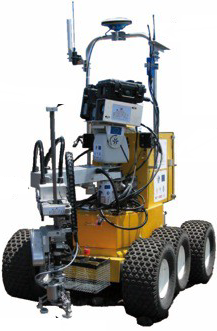
\includegraphics[width=.5\linewidth]{fig_00}}
\def\xxpied{%
\textsf{\xxactivite}%dans le but de déterminer les contraintes géométriques dans les mécanismes\\% afin de valider leurs performances.\\
%Révisions 1 -- 2 -- 3 -- \xxactivite%
}

\def\xxposongletx{2}
\def\xxposonglettext{1.45}
\def\xxposonglety{20}
%\def\xxonglet{Part. 1 -- Ch. 3}


\usepackage{multicol}
\usepackage{siunitx}

\usepackage{tkz-kiviat}
\fichetrue
%\fichefalse


%\newcommand{\progress}[1]{
%    \begin{tikzpicture}
%        \fill[ocre!20, rounded corners =1 mm] (0,0) rectangle (#1/100*2.5,.4);
%         \draw[ocre,thick, rounded corners =1 mm] (0,0) rectangle (2.5,.4);
%         \node at (1.25,0.2) {\textcolor{black}{#1~\%}};
%    \end{tikzpicture}
%}

\proftrue
\proffalse

\tdtrue
\tdfalse

\courstrue
\coursfalse

\setcounter{secnumdepth}{5}
%---------------------------------------------------------------------------


\begin{document}
%\chapterimage{png/Fond_Cin}
\pagestyle{empty}


%%%%%%%% PAGE DE GARDE COURS
\ifcours
\begin{tikzpicture}[remember picture,overlay]
\node at (current page.north west)
{\begin{tikzpicture}[remember picture,overlay]
\node[anchor=north west,inner sep=0pt] at (0,0) {\includegraphics[width=\paperwidth]{\thechapterimage}};
\draw[anchor=west] (-2cm,-8cm) node [line width=2pt,rounded corners=15pt,draw=ocre,fill=white,fill opacity=0.6,inner sep=40pt]{\strut\makebox[22cm]{}};
\draw[anchor=west] (1cm,-8cm) node {\huge\sffamily\bfseries\color{black} %
\begin{minipage}{1cm}
\rotatebox{90}{\LARGE\sffamily\textsc{\color{ocre}\textbf{\xxnumpartie}}}
\end{minipage} \hfill
\begin{minipage}[c]{14cm}
\begin{titrepartie}
\begin{flushright}
\renewcommand{\baselinestretch}{1.1} 
\Large\sffamily\textsc{\textbf{\xxpartie}}
\renewcommand{\baselinestretch}{1} 
\end{flushright}
\end{titrepartie}
\end{minipage} \hfill
\begin{minipage}[c]{3.5cm}
{\large\sffamily\textsc{\textbf{\color{ocre} \discipline}}}
\end{minipage} 
 };
\end{tikzpicture}};
\end{tikzpicture}


\begin{tikzpicture}[overlay]
\node[shape=rectangle, 
      rounded corners = .25 cm,
	  draw= ocre,
	  line width=2pt, 
	  fill = ocre!10,
	  minimum width  = 2.5cm,
	  minimum height = 3cm,] at (18cm,0) {};
\node at (17.7cm,0) {\rotatebox{90}{\textbf{\Large\color{ocre}{\classe}}}};
%{};
\end{tikzpicture}

\vspace{3.5cm}

\begin{tikzpicture}[remember picture,overlay]
\draw[anchor=west] (-2cm,-6cm) node {\huge\sffamily\bfseries\color{black} %
\begin{minipage}{2cm}
\begin{center}
\LARGE\sffamily\textsc{\color{ocre}\textbf{\xxactivite}}
\end{center}
\end{minipage} \hfill
\begin{minipage}[c]{15cm}
\begin{titrechapitre}
\renewcommand{\baselinestretch}{1.1} 
\Large\sffamily\textsc{\textbf{\xxnumchapitre}}

\Large\sffamily\textsc{\textbf{\xxchapitre}}
\vspace{.5cm}

\renewcommand{\baselinestretch}{1} 
\normalsize\normalfont
\xxcompetences
\end{titrechapitre}
\end{minipage}  };
\end{tikzpicture}
\vfill

\begin{flushright}
\begin{minipage}[c]{.3\linewidth}
\begin{center}
\xxfigures
\end{center}
\end{minipage}\hfill
\begin{minipage}[c]{.6\linewidth}
\startcontents
\printcontents{}{1}{}
\end{minipage}
\end{flushright}

\begin{tikzpicture}[remember picture,overlay]
\draw[anchor=west] (4.5cm,-.7cm) node {
\begin{minipage}[c]{.2\linewidth}
\begin{flushright}
\includegraphics[width=2cm]{png/logoCC}
\end{flushright}
\end{minipage}
\begin{minipage}[c]{.2\linewidth}
\textsl{\xxauteur} \\
\textsl{\classe}
\end{minipage}
 };
\end{tikzpicture}
\newpage
\pagestyle{fancy}

\newpage
\pagestyle{fancy}

\else
\fi


%%%%%%%% PAGE DE GARDE TD
\iftd
%\begin{tikzpicture}[remember picture,overlay]
%\node at (current page.north west)
%{\begin{tikzpicture}[remember picture,overlay]
%\draw[anchor=west] (-2cm,-3.25cm) node [line width=2pt,rounded corners=15pt,draw=ocre,fill=white,fill opacity=0.6,inner sep=40pt]{\strut\makebox[22cm]{}};
%\draw[anchor=west] (1cm,-3.25cm) node {\huge\sffamily\bfseries\color{black} %
%\begin{minipage}{1cm}
%\rotatebox{90}{\LARGE\sffamily\textsc{\color{ocre}\textbf{\xxnumpartie}}}
%\end{minipage} \hfill
%\begin{minipage}[c]{13.5cm}
%\begin{titrepartie}
%\begin{flushright}
%\renewcommand{\baselinestretch}{1.1} 
%\Large\sffamily\textsc{\textbf{\xxpartie}}
%\renewcommand{\baselinestretch}{1} 
%\end{flushright}
%\end{titrepartie}
%\end{minipage} \hfill
%\begin{minipage}[c]{3.5cm}
%{\large\sffamily\textsc{\textbf{\color{ocre} \discipline}}}
%\end{minipage} 
% };
%\end{tikzpicture}};
%\end{tikzpicture}

%%%%%%%%%% PAGE DE GARDE TD %%%%%%%%%%%%%%%
%\begin{tikzpicture}[overlay]
%\node[shape=rectangle, 
%      rounded corners = .25 cm,
%	  draw= ocre,
%	  line width=2pt, 
%	  fill = ocre!10,
%	  minimum width  = 2.5cm,
%	  minimum height = 2.5cm,] at (18.5cm,0) {};
%\node at (17.7cm,0) {\rotatebox{90}{\textbf{\Large\color{ocre}{\classe}}}};
%%{};
%\end{tikzpicture}

% PARTIE ET CHAPITRE
%\begin{tikzpicture}[remember picture,overlay]
%\draw[anchor=west] (-1cm,-2.1cm) node {\large\sffamily\bfseries\color{black} %
%\begin{minipage}[c]{15cm}
%\begin{flushleft}
%\xxnumchapitre \\
%\xxchapitre
%\end{flushleft}
%\end{minipage}  };
%\end{tikzpicture}

% Bandeau titre exo
\begin{tikzpicture}[remember picture,overlay]
\draw[anchor=west] (-2cm,-4cm) node {\huge\sffamily\bfseries\color{black} %
\begin{minipage}{5cm}
\begin{center}
\LARGE\sffamily\color{ocre}\textbf{\textsc{\xxactivite}}

\begin{center}
\xxfigures
\end{center}

\end{center}
\end{minipage} \hfill
\begin{minipage}[c]{12cm}
\begin{titrechapitre}
\renewcommand{\baselinestretch}{1.1} 
\large\sffamily\textbf{\textsc{\xxtitreexo}}

\small\sffamily{\textbf{\textit{\color{black!70}\xxsourceexo}}}
\vspace{.5cm}

\renewcommand{\baselinestretch}{1} 
\normalsize\normalfont
\xxcompetences
\end{titrechapitre}
\end{minipage}  };
\end{tikzpicture}

\else
\fi


%%%%%%%% PAGE DE GARDE FICHE
\iffiche
\begin{tikzpicture}[remember picture,overlay]
\node at (current page.north west)
{\begin{tikzpicture}[remember picture,overlay]
\draw[anchor=west] (-2cm,-3.25cm) node [line width=2pt,rounded corners=15pt,draw=ocre,fill=white,fill opacity=0.6,inner sep=40pt]{\strut\makebox[22cm]{}};
\draw[anchor=west] (1cm,-3.25cm) node {\huge\sffamily\bfseries\color{black} %
\begin{minipage}{1cm}
\rotatebox{90}{\LARGE\sffamily\textsc{\color{ocre}\textbf{\xxnumpartie}}}
\end{minipage} \hfill
\begin{minipage}[c]{14cm}
\begin{titrepartie}
\begin{flushright}
\renewcommand{\baselinestretch}{1.1} 
\large\sffamily\textsc{\textbf{\xxpartie} \\} 

\vspace{.2cm}

\normalsize\sffamily\textsc{\textbf{\xxnumchapitre -- \xxchapitre}}
\renewcommand{\baselinestretch}{1} 
\end{flushright}
\end{titrepartie}
\end{minipage} \hfill
\begin{minipage}[c]{3.5cm}
{\large\sffamily\textsc{\textbf{\color{ocre} \discipline}}}
\end{minipage} 
 };
\end{tikzpicture}};
\end{tikzpicture}


\begin{tikzpicture}[overlay]
\node[shape=rectangle, 
      rounded corners = .25 cm,
	  draw= ocre,
	  line width=2pt, 
	  fill = ocre!10,
	  minimum width  = 2.5cm,
	  minimum height = 2.5cm,] at (18.5cm,0.cm) {};
%	  minimum height = 2.5cm,] at (18.5cm,0cm) {};
\node at (17.7cm,0cm) {\rotatebox{90}{\textsf{\textbf{\large\color{ocre}{\classe}}}}};
%{};
\end{tikzpicture}



\else
\fi



%\vspace{4.5cm}
\pagestyle{fancy}
\thispagestyle{plain}


\def\columnseprulecolor{\color{ocre}}
\setlength{\columnseprule}{0pt} 


\begin{tikzpicture}[remember picture,overlay]
\draw[anchor=west] (-2cm,-4cm) node {\huge\sffamily\bfseries\color{black} %
\begin{minipage}{5cm}
\begin{center}
\LARGE\sffamily\color{ocre}\textbf{\textsc{\xxactivite}}

\begin{center}
\xxfigures
\end{center}

\end{center}
\end{minipage} \hfill
\begin{minipage}[c]{12cm}
\begin{titrechapitre}
\renewcommand{\baselinestretch}{1.1} 
\large\sffamily\textbf{\textsc{\xxtitreexo}}

\small\sffamily{\textbf{\textit{\color{black!70}\xxsourceexo}}}
\vspace{.5cm}

\renewcommand{\baselinestretch}{1} 
\normalsize\normalfont
%\xxcompetences
\end{titrechapitre}
\end{minipage}};
\end{tikzpicture}

\vspace{6cm}
%

\textbf{Remarques générales}
\begin{itemize}
\item Ensemble satisfaisant. Les fonctions de bases sont globalement bien codées. 
\item Le cours sur les variants invariants complexité est plutôt bien appréhendé. 
\item Les questions sur la bordure ont eu un succès très mitigé. Il s'agissait d'ajouter une bordure et pas de remplacer les pixels du bords par des pixels noirs. 
\end{itemize}


\begin{minipage}[c]{.45\linewidth} 
\Large \textbf{\textsf{XXXXX XXXxxxxxx}} 
 
 \normalsize Note brute 6.65/20 
 
 \normalsize Note harmonisée 9.31/20 
 
Rang 27
 
Moyenne classe brute 6.75/20 
 
Moyenne question traitées 8.31/20 
 
Rang question traitées 32 
 
Commentaires : 
Un ensemble un peu inégal. Sur ce genre de sujet, il ne faut traiter de manière exhaustive les questions abordées.(Pour le cahier des charges, il faut par exemple évaluer chacun des critères).  
\end{minipage}\hfill 
\begin{minipage}[c]{.45\linewidth}  
\begin{center}
\includegraphics[width=.8\linewidth]{../histo.pdf} 
\end{center}
\end{minipage}
\footnotesize 
\begin{center} 
\begin{tabular}{|c|c|m{1cm}|c||c|c|m{1cm}|c||c|c|m{1cm}|c||c|c|m{1cm}|c|} 
\hline \textbf{Qu} & \textbf{Coef} & \textbf{Comp} & \textbf{/5} & \textbf{Qu} & \textbf{Coef} & \textbf{Comp} & \textbf{/5} & \textbf{Qu} & \textbf{Coef} & \textbf{Comp} & \textbf{/5} & \textbf{Qu} & \textbf{Coef} & \textbf{Comp} & \textbf{/5} \\ 
\hline 
\hline 
Q1 & 1 & GEO-01 & 3.5 & Q1 & 2 & GEO-02 & NT & Q2 & 1 & GEO-03 & 0 & Q3 & 2 & GEO-04 & 2 \\ \hline 
 
Q3 & 1 & CIN-01 & 0 & Q4 & 2 & CIN-02 & 0 & Q5 & 1 & CIN-03 & 3 & Q6 & 2 & CIN-04 & 2 \\ \hline 
 
Q7 & 1 & CIN-05 & 5 & Q8 & 2 & STAT-01 & 4 & Q9 & 1 & STAT-02 & NT & Q10 & 2 & STAT-03 & 0 \\ \hline 
 
Q11 & 1 & STAT-04 & 0 & Q12 & 2 & STAT-05 & 5 & Q13 & 1 & CHS-01 & 5 & Q14 & 2 & CHS-02 & 5 \\ \hline 
 
Q15 & 1 & CHS-03 & 0 & Q16 & 2 & CHS-04 & 0 & Q17 & 1 & CHS-05 & NT & Q18 & 2 & DYN-01 & NT \\ \hline 
 
Q19 & 1 & DYN-02 & 1 & Q20 & 2 & DYN-03 & 4 & Q21 & 1 & DYN-04 & 3 & Q22 & 2 & DYN-05 & 1 \\ \hline 
 
Q23 & 1 & DYN-06 & 0 & Q24 & 2 & TEC-01 & NT & Q24 & 1 & TEC-02 & 0 &  &  &  &  \\ \hline 
 
\end{tabular} 
\end{center} 
\normalsize 
 
\noindent \textbf{Bilan par compétences}
 
\begin{itemize} 
\item  \footnotesize \xpComp{CHS}{01} \normalsize \hspace{.2cm}Analyser un mécanisme en utilisant un graphe de liaisons\hfill \progress{100}
\item  \footnotesize \xpComp{CHS}{02} \normalsize \hspace{.2cm}Simplifier un mécanisme en utilisant une liaison équivalente\hfill \progress{100}
\item  \footnotesize \xpComp{CHS}{03} \normalsize \hspace{.2cm}Evaluer l'hyperstatisme d'un mécanisme\hfill \progress{0}
\item  \footnotesize \xpComp{CHS}{04} \normalsize \hspace{.2cm}Simplifier un mécanisme pour le rendre isostatique\hfill \progress{0}
\item  \footnotesize \xpComp{CHS}{05} \normalsize \hspace{.2cm}Analyser les conséquences de l'hyperstatisme d'un mécanisme\hfill \progress{0}
\item  \footnotesize \xpComp{CIN}{01} \normalsize \hspace{.2cm}Analyser un mécanisme, réaliser un graphe de liaison\hfill \progress{0}
\item  \footnotesize \xpComp{CIN}{02} \normalsize \hspace{.2cm}Déterminer un vecteur vitesse, un torseur cinématique, un vecteur accélération\hfill \progress{0}
\item  \footnotesize \xpComp{CIN}{03} \normalsize \hspace{.2cm}Déterminer le rapport de transmission d'un transmetteur\hfill \progress{60}
\item  \footnotesize \xpComp{CIN}{04} \normalsize \hspace{.2cm}Déterminer un loi ES cinématique, utiliser l'hypothèse de RSG\hfill \progress{40}
\item  \footnotesize \xpComp{CIN}{05} \normalsize \hspace{.2cm}Evaluer expérimentalement une grandeur cinématique\hfill \progress{100}
\item  \footnotesize \xpComp{DYN}{01} \normalsize \hspace{.2cm}Analyser un problème, définir une loi de mouvement \hfill \progress{0}
\item  \footnotesize \xpComp{DYN}{02} \normalsize \hspace{.2cm}Analyser un mécanisme en utilisant un graphe de structure\hfill \progress{20}
\item  \footnotesize \xpComp{DYN}{03} \normalsize \hspace{.2cm}Modéliser un solide et déterminer ses caractéristiques inertielles\hfill \progress{80}
\item  \footnotesize \xpComp{DYN}{04} \normalsize \hspace{.2cm}Déterminer un torseur cinétique, un torseur dynamique\hfill \progress{60}
\item  \footnotesize \xpComp{DYN}{05} \normalsize \hspace{.2cm}Proposer une démarche de résolution en utilisant le PFD\hfill \progress{20}
\item  \footnotesize \xpComp{DYN}{06} \normalsize \hspace{.2cm}Mettre en œuvre une démarche de résolution en utilisant le PFD\hfill \progress{0}
\item  \footnotesize \xpComp{GEO}{01} \normalsize \hspace{.2cm}Analyser la géométrie d'un mécanisme, analyser des surfaces de contact, réaliser des constructions géométriques\hfill \progress{70}
\item  \footnotesize \xpComp{GEO}{02} \normalsize \hspace{.2cm}Modéliser un mécanisme en réalisant un schéma cinématique paramétré\hfill \progress{0}
\item  \footnotesize \xpComp{GEO}{03} \normalsize \hspace{.2cm}Résoudre un problème de géométrie : déterminer la trajectoire d'un point ou déterminer une loi Entrée - Sortie\hfill \progress{0}
\item  \footnotesize \xpComp{GEO}{04} \normalsize \hspace{.2cm}Evaluer expérimentalement des grandeurs géométriques\hfill \progress{40}
\item  \footnotesize \xpComp{STAT}{01} \normalsize \hspace{.2cm}Analyser un problème en utilisant un graphe de structure\hfill \progress{80}
\item  \footnotesize \xpComp{STAT}{02} \normalsize \hspace{.2cm}Modéliser les actions mécaniques locales, globales, frottement\hfill \progress{0}
\item  \footnotesize \xpComp{STAT}{03} \normalsize \hspace{.2cm}Proposer une démarche de résolution en utilisant le PFS\hfill \progress{0}
\item  \footnotesize \xpComp{STAT}{04} \normalsize \hspace{.2cm}Mettre en œuvre une démarche de résolution\hfill \progress{0}
\item  \footnotesize \xpComp{STAT}{05} \normalsize \hspace{.2cm}Evaluer expérimentalement une action mécanique\hfill \progress{100}
\item  \footnotesize \xpComp{TEC}{01} \normalsize \hspace{.2cm}Analyser un mécanisme en utilisant un graphe de structure\hfill \progress{0}
\item  \footnotesize \xpComp{TEC}{02} \normalsize \hspace{.2cm}Déterminer les puissances intérieures\hfill \progress{0}
\end{itemize} 
\newpage 
\textbf{Bilan de compétences} 

\begin{minipage}[c]{.3\linewidth} 
\begin{tikzpicture}[scale=1, label distance = .5cm]
    \tkzKiviatDiagram[lattice=5,gap=.3,space=.3,step=1,radial style/.style ={-latex},lattice style/.style ={blue!30}]{SYS-01,SYS-02,SYS-03,SYS-04,SYS-05,SYS-06}
    \tkzKiviatLine[thick,color=red,mark=ball,ball color=red,mark size=3pt,fill=red!20](0.0,0.0,0.0,0.0,1.0000000000000002,4.0)
    \tkzKiviatLine[very thick, dotted, color=blue,mark=ball,mark size=1pt,fill=blue!20,	opacity=.5](1.857142857142857,1.7500000000000004,0.7142857142857144,1.25,1.8809523809523807,1.4047619047619047)
\end{tikzpicture} 
\end{minipage}\hfill 
\begin{minipage}[c]{.6\linewidth} 
\footnotesize 
\allSysComp
\normalsize 
\end{minipage} 
\begin{minipage}[c]{.3\linewidth} 
\begin{tikzpicture}[scale=1, label distance = .5cm]
    \tkzKiviatDiagram[lattice=5,gap=.3,space=.3,step=1,radial style/.style ={-latex},lattice style/.style ={blue!30}]{GEO-01,GEO-02,GEO-03,GEO-04}
    \tkzKiviatLine[thick,color=red,mark=ball,ball color=red,mark size=3pt,fill=red!20](3.1666666666666665,0.6000000000000001,0.0,1.0)
    \tkzKiviatLine[very thick, dotted, color=blue,mark=ball,mark size=1pt,fill=blue!20,	opacity=.5](1.2110317460317455,1.1666666666666667,0.8333333333333335,0.9464285714285713)
\end{tikzpicture} 
\end{minipage}\hfill 
\begin{minipage}[c]{.6\linewidth} 
\footnotesize 
\allGeoComp
\normalsize 
\end{minipage} 
\begin{minipage}[c]{.3\linewidth} 
\begin{tikzpicture}[scale=1, label distance = .5cm]
    \tkzKiviatDiagram[lattice=5,gap=.3,space=.3,step=1,radial style/.style ={-latex},lattice style/.style ={blue!30}]{CIN-01,CIN-02,CIN-03,CIN-04,CIN-05}
    \tkzKiviatLine[thick,color=red,mark=ball,ball color=red,mark size=3pt,fill=red!20](0.7,0.0,0.75,2.0000000000000004,1.6666666666666665)
    \tkzKiviatLine[very thick, dotted, color=blue,mark=ball,mark size=1pt,fill=blue!20,	opacity=.5](1.055190476190476,1.2023809523809528,1.2232142857142863,1.9826984126984124,1.654761904761905)
\end{tikzpicture} 
\end{minipage}\hfill 
\begin{minipage}[c]{.6\linewidth} 
\footnotesize 
\allCinComp
\normalsize 
\end{minipage} 
\begin{minipage}[c]{.3\linewidth} 
\begin{tikzpicture}[scale=1, label distance = .5cm]
    \tkzKiviatDiagram[lattice=5,gap=.3,space=.3,step=1,radial style/.style ={-latex},lattice style/.style ={blue!30}]{STAT-01,STAT-02,STAT-03,STAT-04,STAT-05}
    \tkzKiviatLine[thick,color=red,mark=ball,ball color=red,mark size=3pt,fill=red!20](1.6,1.5,1.0,3.75,4.666666666666666)
    \tkzKiviatLine[very thick, dotted, color=blue,mark=ball,mark size=1pt,fill=blue!20,	opacity=.5](1.926190476190476,1.6964285714285716,1.9423809523809528,2.4732142857142856,3.1626984126984126)
\end{tikzpicture} 
\end{minipage}\hfill 
\begin{minipage}[c]{.6\linewidth} 
\footnotesize 
\allStatComp
\normalsize 
\end{minipage} 
\begin{minipage}[c]{.3\linewidth} 
\begin{tikzpicture}[scale=1, label distance = .5cm]
    \tkzKiviatDiagram[lattice=5,gap=.3,space=.3,step=1,radial style/.style ={-latex},lattice style/.style ={blue!30}]{CHS-01,CHS-02,CHS-03,CHS-04,CHS-05}
    \tkzKiviatLine[thick,color=red,mark=ball,ball color=red,mark size=3pt,fill=red!20](1.6666666666666665,2.0,0.0,2.5,3.75)
    \tkzKiviatLine[very thick, dotted, color=blue,mark=ball,mark size=1pt,fill=blue!20,	opacity=.5](2.6944444444444446,2.0142857142857147,2.500000000000001,2.440476190476192,2.383928571428572)
\end{tikzpicture} 
\end{minipage}\hfill 
\begin{minipage}[c]{.6\linewidth} 
\footnotesize 
\allChsComp
\normalsize 
\end{minipage} 
\begin{minipage}[c]{.3\linewidth} 
\begin{tikzpicture}[scale=1, label distance = .5cm]
    \tkzKiviatDiagram[lattice=5,gap=.3,space=.3,step=1,radial style/.style ={-latex},lattice style/.style ={blue!30}]{DYN-01,DYN-02,DYN-03,DYN-04,DYN-05,DYN-06}
    \tkzKiviatLine[thick,color=red,mark=ball,ball color=red,mark size=3pt,fill=red!20](1.6666666666666665,0.3333333333333333,1.6,1.5,0.5,0.7500000000000001)
    \tkzKiviatLine[very thick, dotted, color=blue,mark=ball,mark size=1pt,fill=blue!20,	opacity=.5](1.630952380952381,1.8650793650793651,1.6119047619047622,0.6071428571428572,1.1488095238095237,1.4880952380952381)
\end{tikzpicture} 
\end{minipage}\hfill 
\begin{minipage}[c]{.6\linewidth} 
\footnotesize 
\allDynComp
\normalsize 
\end{minipage} 
\begin{minipage}[c]{.3\linewidth} 
\begin{tikzpicture}[scale=1, label distance = .5cm]
    \tkzKiviatDiagram[lattice=5,gap=.3,space=.3,step=1,radial style/.style ={-latex},lattice style/.style ={blue!30}]{TEC-01,TEC-02,TEC-03,TEC-04,TEC-05}
    \tkzKiviatLine[thick,color=red,mark=ball,ball color=red,mark size=3pt,fill=red!20](2.2,0.9999999999999999,0.7500000000000001,1.3333333333333333,0.0)
    \tkzKiviatLine[very thick, dotted, color=blue,mark=ball,mark size=1pt,fill=blue!20,	opacity=.5](1.4103809523809518,0.9107142857142859,1.1249999999999998,1.2380952380952377,0.8904761904761905)
\end{tikzpicture} 
\end{minipage}\hfill 
\begin{minipage}[c]{.6\linewidth} 
\footnotesize 
\allTecComp
\normalsize 
\end{minipage} 
\begin{minipage}[c]{.3\linewidth} 
\begin{tikzpicture}[scale=1, label distance = .5cm]
    \tkzKiviatDiagram[lattice=5,gap=.3,space=.3,step=1,radial style/.style ={-latex},lattice style/.style ={blue!30}]{SLCI-01,SLCI-02,SLCI-03,SLCI-04,SLCI-05,SLCI-06,SLCI-07,SLCI-08,SLCI-09,SLCI-10,SLCI-11}
    \tkzKiviatLine[thick,color=red,mark=ball,ball color=red,mark size=3pt,fill=red!20](1.4999999999999996,1.5,1.5000000000000002,2.75,2.0,0.0,2.25,1.0,5.0,4.25,2.5)
    \tkzKiviatLine[very thick, dotted, color=blue,mark=ball,mark size=1pt,fill=blue!20,	opacity=.5](1.4635034013605437,1.083333333333333,1.931428571428572,1.8392857142857144,2.291666666666666,2.1934523809523805,1.056547619047619,2.6328571428571435,2.9107142857142856,3.154761904761904,2.4821428571428577)
\end{tikzpicture} 
\end{minipage}\hfill 
\begin{minipage}[c]{.6\linewidth} 
\footnotesize 
\allSlciComp
\normalsize 
\end{minipage} 
\begin{minipage}[c]{.3\linewidth} 
\begin{tikzpicture}[scale=1, label distance = .5cm]
    \tkzKiviatDiagram[lattice=5,gap=.3,space=.3,step=1,radial style/.style ={-latex},lattice style/.style ={blue!30}]{PERF-01,PERF-02,PERF-03,PERF-04,PERF-05,PERF-06}
    \tkzKiviatLine[thick,color=red,mark=ball,ball color=red,mark size=3pt,fill=red!20](0.0,0.0,3.0,1.25,3.666666666666667,1.6)
    \tkzKiviatLine[very thick, dotted, color=blue,mark=ball,mark size=1pt,fill=blue!20,	opacity=.5](1.8333333333333335,2.678571428571429,2.164285714285716,1.6726190476190474,2.2222222222222223,1.6761904761904767)
\end{tikzpicture} 
\end{minipage}\hfill 
\begin{minipage}[c]{.6\linewidth} 
\footnotesize 
\allPerfComp
\normalsize 
\end{minipage} 
\begin{minipage}[c]{.3\linewidth} 
\begin{tikzpicture}[scale=1, label distance = .5cm]
    \tkzKiviatDiagram[lattice=5,gap=.3,space=.3,step=1,radial style/.style ={-latex},lattice style/.style ={blue!30}]{COR-01,COR-02,COR-03,COR-04,COR-05,COR-06}
    \tkzKiviatLine[thick,color=red,mark=ball,ball color=red,mark size=3pt,fill=red!20](2.5,0.2,0.0,0.6000000000000001,1.6,1.5)
    \tkzKiviatLine[very thick, dotted, color=blue,mark=ball,mark size=1pt,fill=blue!20,	opacity=.5](1.1766190476190475,1.0333333333333334,1.055059523809524,0.830952380952381,1.1904761904761905,0.7797619047619044)
\end{tikzpicture} 
\end{minipage}\hfill 
\begin{minipage}[c]{.6\linewidth} 
\footnotesize 
\allCorComp
\normalsize 
\end{minipage} 
\begin{minipage}[c]{.3\linewidth} 
\begin{tikzpicture}[scale=1, label distance = .5cm]
    \tkzKiviatDiagram[lattice=5,gap=.3,space=.3,step=1,radial style/.style ={-latex},lattice style/.style ={blue!30}]{NL-01,NL-02}
    \tkzKiviatLine[thick,color=red,mark=ball,ball color=red,mark size=3pt,fill=red!20](2.0,1.0)
    \tkzKiviatLine[very thick, dotted, color=blue,mark=ball,mark size=1pt,fill=blue!20,	opacity=.5](0.9345238095238094,1.2161904761904763)
\end{tikzpicture} 
\end{minipage}\hfill 
\begin{minipage}[c]{.6\linewidth} 
\footnotesize 
\allNlComp
\normalsize 
\end{minipage} 
\begin{minipage}[c]{.3\linewidth} 
\begin{tikzpicture}[scale=1, label distance = .5cm]
    \tkzKiviatDiagram[lattice=5,gap=.3,space=.3,step=1,radial style/.style ={-latex},lattice style/.style ={blue!30}]{SEQ-01,SEQ-02,SEQ-03}
    \tkzKiviatLine[thick,color=red,mark=ball,ball color=red,mark size=3pt,fill=red!20](2.5,2.0,0.0)
    \tkzKiviatLine[very thick, dotted, color=blue,mark=ball,mark size=1pt,fill=blue!20,	opacity=.5](1.2202380952380951,1.8273809523809528,2.5714285714285716)
\end{tikzpicture} 
\end{minipage}\hfill 
\begin{minipage}[c]{.6\linewidth} 
\footnotesize 
\allSeqComp
\normalsize 
\end{minipage} 
\begin{minipage}[c]{.3\linewidth} 
\begin{tikzpicture}[scale=1, label distance = .5cm]
    \tkzKiviatDiagram[lattice=5,gap=.3,space=.3,step=1,radial style/.style ={-latex},lattice style/.style ={blue!30}]{NUM-01,NUM-02,NUM-03,NUM-04,NUM-05}
    \tkzKiviatLine[thick,color=red,mark=ball,ball color=red,mark size=3pt,fill=red!20](0.0,0.0,5.0,5.0,5.0)
    \tkzKiviatLine[very thick, dotted, color=blue,mark=ball,mark size=1pt,fill=blue!20,	opacity=.5](1.7619047619047619,3.142857142857143,3.1309523809523823,2.9404761904761907,2.392857142857143)
\end{tikzpicture} 
\end{minipage}\hfill 
\begin{minipage}[c]{.6\linewidth} 
\footnotesize 
\allNumComp
\normalsize 
\end{minipage} 






\end{document}
